\documentclass[12pt]{article}
\usepackage[utf8]{inputenc}
\usepackage{parskip}
\usepackage[a4paper, margin=1.5in]{geometry}
\usepackage{graphicx}
\usepackage[hidelinks]{hyperref}
\usepackage{listings}
\usepackage{array}
\usepackage{minted}
\usepackage{enumitem}
\usepackage{pdfpages}
\usepackage{wrapfig}
\usepackage{amsmath}
\usepackage{cleveref}
\usepackage{subcaption}

\usepackage{blindtext}

\renewcommand{\arraystretch}{1.5}

\begin{document}

\begin{titlepage}

\begin{figure}[t]
	\centering\includegraphics[width=0.9\textwidth]{immagini/marchio_unipi_pant541.eps}
\end{figure}

\begin{center}
	\textbf{Master of Science in Computer Engineering\\}
	\vspace{30mm}
    {\Huge{\bf {Project Report}}}\\
    \vspace{10mm}
    {\Huge{\bf {Control Tower}}}\\
	\vspace{10mm}
	{\LARGE{\bf Performance Evaluation\\[0.5em]of Computer Systems and Networks}}\\
    \vspace{20mm}
\end{center}

\vspace{8mm}

\begin{center}
	{\large Federico Fregosi, Tommaso Billi, Antonio Nunzio Pio Di Noia}
\end{center}

\vfill

\centering{\large{\bf Academic Year 2021/2022 }}

\end{titlepage}

\pagenumbering{gobble}

\tableofcontents
\vfill
\clearpage
\setcounter{page}{1}
\pagenumbering{arabic}

\section{Introduction}
\subsection{Overview}
Consider a system that mimics an airport. The airport consists of one runway, a parking area and a control tower. The runway is used for landing/take-off and can be occupied by only one plane at a time, whereas the parking area has infinite capacity. The control tower manages the air traffic of the airport; each airplane follows the following steps to enter and leave the airport:
\begin{enumerate}
    \item it queues for landing;
    \item it lands on the runway;
    \item it moves in the parking lot and stay here for a certain time;
    \item it queues for take-off;
    \item it takes-off and leave the airport.
\end{enumerate}
Landing and take-off operations, as well as parking, require a specific time for each airplane. In particular, for each plane we have:
\begin{itemize}
    \item $t_l$ = time necessary to perform the landing operation;
	\item $t_p$ = time that the airplane will spend in the parking area;
	\item $t_o$ = time necessary to perform the take-off operation.
\end{itemize}
When the runway is occupied, planes that are required to land or take off are placed respectively in the landing queue or in the take-off queue. The queues are FIFO, and their capacity is assumed to be unlimited. When the runway is unoccupied instead, the control tower serves one airplane from a queue, prioritizing take-off over landing; planes in the landing queue are served only when the take-off queue is empty. Whenever a plane takes off, it leaves the system.

\subsection{Objectives}
In this analysis, the following objectives will be investigated:
\begin{itemize}
	\item relationship between the service times and the waiting time in both landing and take-off queues: in the system we assume that airplanes have infinite fuel, while in a real environment airplanes have instead a finite quantity of fuel. Studies in the waiting time can be used to estimate the quantity of fuel needed in order to stay in the air until clearance for landing is received;
	\item optimal value for the size of the parking area: we want a good estimation of the space required to accommodate parked planes, without wasting too much of it.
\end{itemize}

\subsection{Performance indexes}
In order to fulfill the above-stated objectives, the following performance indexes will be taken into consideration:
\begin{itemize}
	\item waiting time for the landing queue
	\item waiting time for the take-off queue
	\item number of airplanes in the parking area
\end{itemize}
To evaluate the state of the system and distinguish the transition state from the steady state, we also used as an index the throughput of the runway.

\subsection{Scenarios}
The following scenarios will be taken into consideration:
\begin{itemize}
	\item constant interarrival times, constant service times (only for code verification since in this scenario queuing is of little interest);
	\item exponential distribution of interarrival times, exponential distribution of service times.
\end{itemize}
%where interarrival times are the times at which a plane ask for landing, whereas service times are the time required for landing, the time required for take-off and the time spent in the parking area.

\section{Model}
\subsection{Description}

\begin{figure}[ht!]
    \centering
    \includegraphics[scale=0.8]{immagini/system_model.jpg}
    \caption{Schematic representation of the model of the system}
    \label{Fig:model}
\end{figure}

In \cref{Fig:model} you can see our model of the system, where:
\begin{itemize}
    \item $\lambda_V$ is the average arrival rate for airplanes that need for landing;
    \item the path is unique: the only possible outgoing arc from the Runway is the one with the same colour of the incoming arc;
    \item the average service rate of the Runway is $\mu_l$ for the landing operation (blue lines) and $\mu_o$ for the take-off operation;
    \item both queues are FIFO;
    \item the Parking Area is a delay center with infinite space, where $\mu_p$ average service rate.
\end{itemize}

\subsubsection{Assumptions}
The following assumptions were made when modeling the system:
\begin{itemize}
	\item infinite queuing space: there is no upper bound in the number of planes in a queue;
	\item infinite parking space: the parking area is composed of infinite servers;
	\item no overtaking: planes cannot change their position in queue;
	\item all the service times of a planes are independent RVs.
	\item messages exchanged between the control tower and the planes have no delay;
	\item no additional runway for taxiing: landing and take-off operations include taxiing procedures.
\end{itemize}

\subsubsection{Stochastic model}\label{stoch}

Defining an accurate queuing theory model for the system proved to be difficult, as it is made of two distinct queues that share a service center (with different service rates), and whose interarrival rates are non-independent.

For this reason, to study the waiting times in the queues we designed a simplified model, that can be obtained from the real model in figure \ref{Fig:model} by applying these two modifications:
\begin{itemize}
    \item removing the parking area from the picture, which acts as a buffer between the queues;
    \item consider a mean interarrival rate at the take-off queue equal to $\lambda_v$.
\end{itemize}

With these two considerations, and by taking into account the priority that the take-off queue has over the landing queue, we can predict the performance indexes for the two queues, as long as the utilization of the runway $\rho$ is sufficiently low.

We denote $\rho_i = \dfrac{\lambda_v}{\mu_i} = \dfrac{t_i}{t_v}$ the runway utilization per queue. Since the take-off queue is not serving planes only in case the landing queue is serving one already, its response time can be computed as the following:
\begin{equation}
    E[R_T] = \dfrac{1}{\mu_o - \lambda_v} + \rho_l \cdot \dfrac{1}{\mu_l} \text{,}
    \label{r-t}
\end{equation}
where the first term is the mean response time in an M/M/1 system, and the second is the probability that the runway is occupied by a landing plane, multiplied by the average landing time. The mean waiting time can be computed as $E[W_T] = E[R_T] - t_o$.

By applying Little's Law, we can compute $E[N_T] = E[R_T] \cdot \lambda_v = \dfrac{E[R_T]}{t_v}$. By observing that the landing queue is serving planes only when the take-off queue is empty, and the runway is free, its mean response time can be estimated as the following:
\begin{equation}
    E[R_L] = \dfrac{1}{\mu_l - \lambda_v} + E[N_T] \cdot E[R_T] \cdot \sum_{n=0}^{+\infty} \rho_t^n = \dfrac{1}{\mu_l - \lambda_v} + E[N_T] \cdot E[R_T] \cdot \dfrac{1}{1 - \rho_t} \text{,}
    \label{r-l}
\end{equation}
where the second term is accounting for the fact that an arriving plane will have to wait that all planes in the take-off queue have been served, before it can land. During this time, more planes could queue up for take-off (this expected number can be computed by multiplying $E[N_T]$ by $\rho_t$), which would still have priority over landing planes. Again, during this wait, even more planes could earn priority over landing ones, and so on. Since we're interested in the behavior of the system in stable conditions $\rho_t < 1$, which means that the infinite sum always converges.

Finally, the waiting time can be trivially computed as $E[W_L] = E[R_L] - t_l$.

\subsection{Factors}
The factors that can affect the modeled system are:
\begin{itemize}
    \item interarrival time of airplanes: $t_v = \tfrac{1}{\lambda_v}$
    \item landing service time: $t_l = \tfrac{1}{\mu_l}$
    \item parking service time: $t_p = \tfrac{1}{\mu_p}$
    \item take-off service time: $t_o = \tfrac{1}{\mu_o}$
\end{itemize}

\section{Implementation}
\subsection{Code Overview}
The model is composed by three nodes:
\begin{itemize}
	\item \textbf{Airspace}: the node in which planes are created and initialized before reaching the control tower asking for a landing operation
	\item  \textbf{Control tower}: the main node of the system. It is responsible for the manage of both landing and take-off queues and operations
	\item  \textbf{Parking area}: node in which planes spend the $t_p$ time
\end{itemize}
Note that the runway isn't a node itself, but it is included into the control tower.

Planes are modeled as messages. They contain information regarding the service times for the three operations that it will need to perform, that are generated whenever a new Airplane message is spawned by the Airspace module.

Although the probability of multiple events happening at the same time is almost negligible in stochastic scenarios, such eventuality must be taken into account. To make sure that the priority between the two queues is maintained even in these case, a different priority was assigned to each type of message that is sent among the modules of the system (from highest to lowest):
\begin{enumerate}[label=\arabic*)]
	\item airplane message leaving the parking area and moving to the take-off queue;
	\item message from the control tower giving the OK and starting the take-off operation;
	\item airplane message spawned from the airspace and moving to the control tower;
	\item message from the control tower giving the OK and starting the landing operation;
	\item self-messages for checking the queues after a take-off or landing operation.
\end{enumerate}

\begin{figure}[H]
    \centering
    \includegraphics[scale=0.45]{immagini/lifecycle}
    \caption{Life-cycle of each airplane}
    \label{Fig:life-cycle of each airplane}
\end{figure}

\subsection{Validation}

\subsubsection{Continuity Test}

This test is about checking that if input\textsubscript{i} produces output\textsubscript{i} then slightly changing the input does not change the output wildly.
As input it was considered the interarrival time of the airplanes, as output their response times. 
Before actually carrying out the continuity test the value of interarrival time for which the system reaches a steady state was found, by fixing all the service times (t\textsubscript{l}, t\textsubscript{p}, t\textsubscript{o}) to constant reasonable, i.e. "realistic" values:

\begin{itemize}
    \item t\textsubscript{l}: 900 seconds = 15 minutes
    \item t\textsubscript{p}: 3600 seconds = 1 hour
    \item t\textsubscript{o}: 900 seconds = 15 minutes
\end{itemize}

For the system to be stable, the interarrival time must be $ t_v > t_l + t_o $, so, taking some safety margin, the lowest value used to carry out this test was 2700 seconds (45 minutes).
The interarrival time range upon which the test was carried out was the following: 

\begin{gather*}
    iat = \{2700 \text{ s}, 2760 \text{ s}, 2820 \text{ s}, 2880 \text{ s}, 2940 \text{ s}, 3000 \text{ s}, 10000 \text{ s}\}
\end{gather*} 

where the value 10,000 was inserted only to show the monotonic behavior of the output, as it should be:
as the interarrival time increases there will be less planes competing at the same time for the single runway, so the response time decreases. 

The result is shown in Figure \ref{continuity_test}.

\begin{figure}[H]
	\centering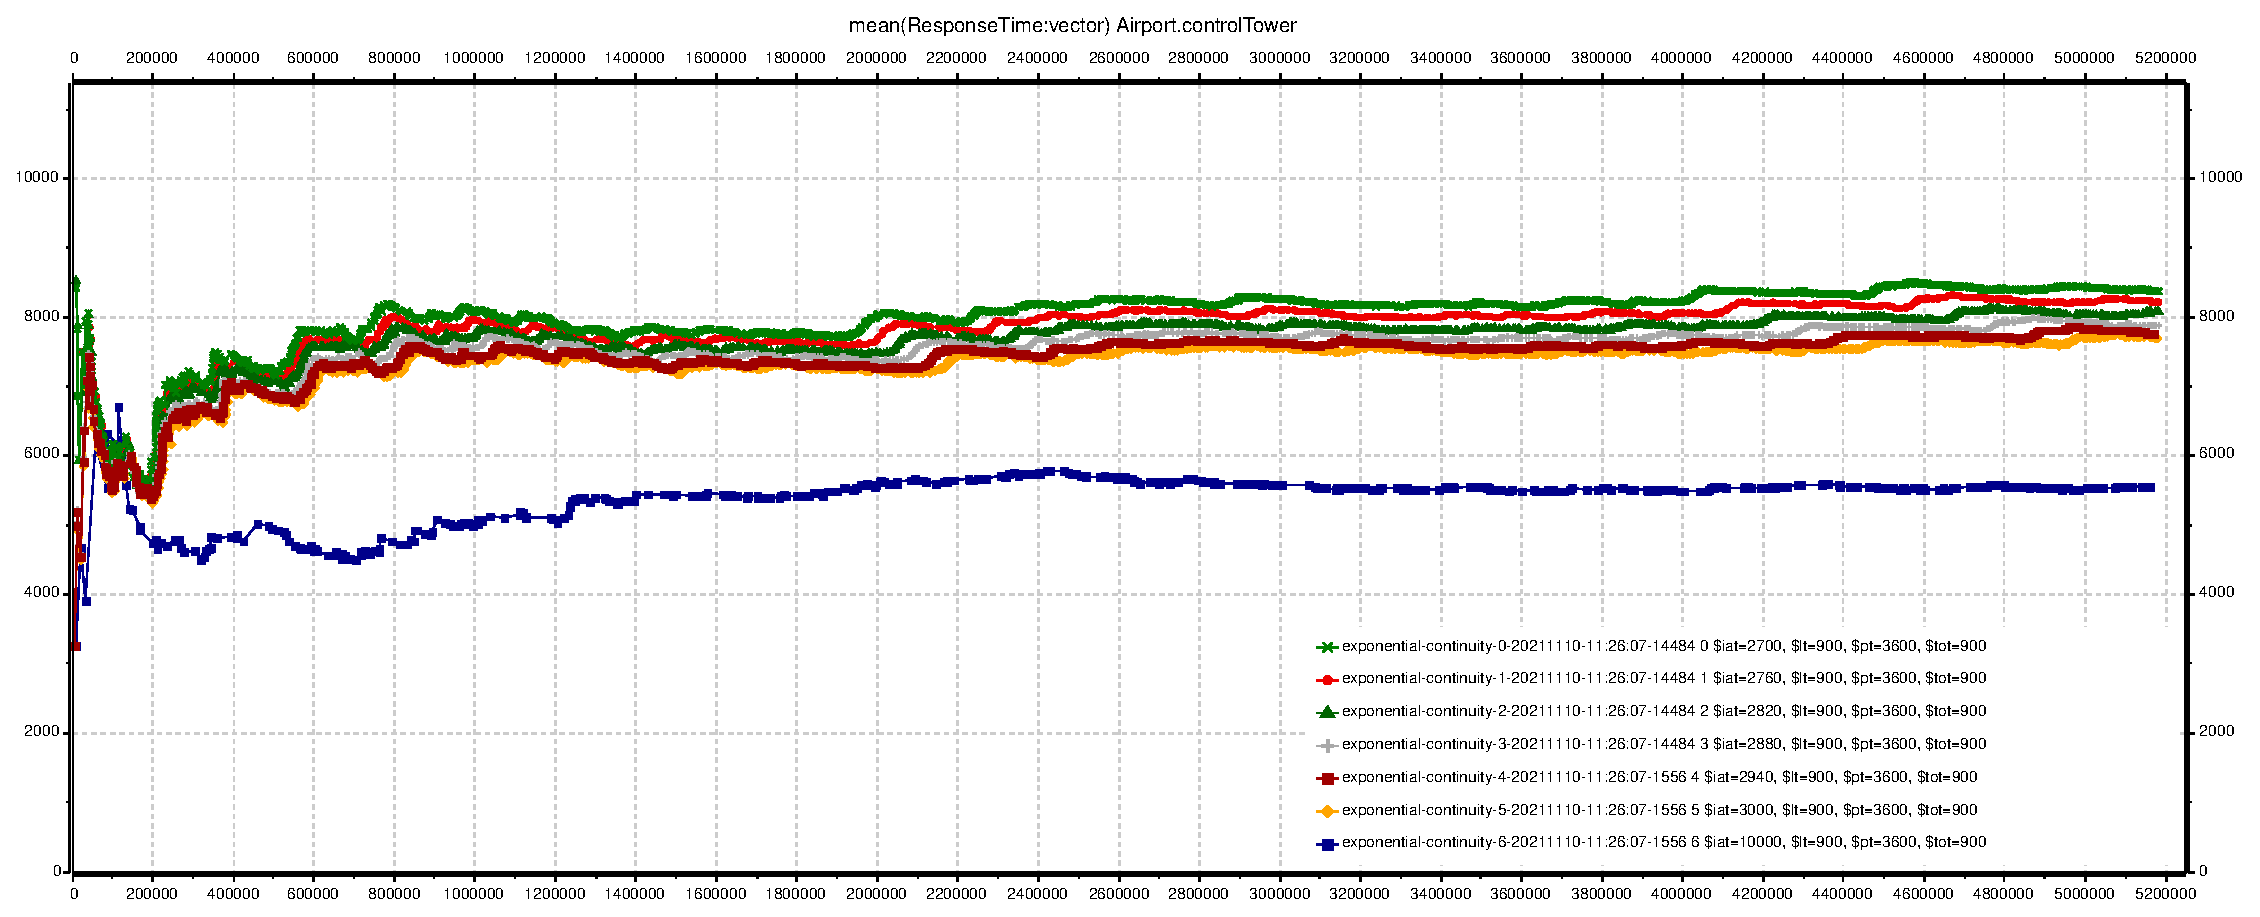
\includegraphics[width=1\textwidth]{immagini/exponential-continuity.eps}
	\caption{Continuity test.}\label{continuity_test}
\end{figure}

\subsection{Preliminary calibration}
\label{preliminary_calibration}

In order to define the set of parameters to be used in the following simulations, we studied the mean response time as a function of the mean interarrival time of planes, for different combinations of service times.

The results that emerged from our study, as we expected, showed that if $t_v < t_l + t_o$, $E[R]$ rapidly increases, as a consequence of the landing queue growing indefinitely. If instead $t_v > t_l + t_o$, the mean response time tends to quickly stabilize around a constant value. Another result that emerged from our tests is that the average time spent in the parking area acts as an additive constant for $E[R]$. This is exactly what we would expect, as no queuing occurs in the parking area, and the mean service time for a delay center is $t_p$.

Having fixed the $t_l$ and $t_o$ service times at 900s, to find a lower bound for the mean interarrival time we computed 95\% confidence intervals for the mean response time over 20 independent repetitions, and found that $t_v \geq 2400\text{s}$ yields a relative margin of error below 2\%, hence we picked $t_v = 2400\text{s}$ as the mean interarrival time for the worst case in the following studies.

To calibrate the system, the following factor ranges were defined:
\begin{itemize}
    \item $t_l \in$ [300s, 900s]
    \item $t_p \in$ [3600s, 36000s]
    \item $t_o \in$ [300s, 900s]
    \item  $t_v \in$ [2400s, 7200s]
\end{itemize}


\subsubsection{Calibration of warm-up period and simulation duration}
In order to define the required warm-up period, we plotted the sliding window average of the response time as a function of the simulation time for 20 different runs. The runs were configured in order to represent a worst-case scenario: $t_l$=900s, $t_p$=36000s, $t_o$=900s,  $\frac{1}{\lambda_v}$=2400s, where the value chosen for lambda is explained in section \ref{preliminary_calibration}.
We carried out the warm-up analysis both on the response time and on the throughput, anyway the the value produced through the study on the response time was larger and so it was chosen as worst case, and it is the one shown in Figure \ref{warm_up_analysis}.

\begin{figure}[H]
	\centering
	\includegraphics[width=.8\textwidth]{report/immagini/exponential-warmup}
	\caption{Study on warm-up.}\label{warm_up_analysis}
\end{figure}

As it can be noted, the plot starts converging at 200.000s, and so, taking a safety margin, a value of 432.000s (= 5 days) was chosen to be used in all the subsequent experiments.

As for the simulation time, a value of 100 days was chosen. This value has to be chosen as a trade-off between the required number of data, and of the time and memory consumption. 
Since the simulator reported in this work is not too much memory/time demanding to be run, a large value for the simulation time was preferred. Also, a study on the standard deviation has been carried out on the response time and other performance indexes, where of course a smaller and more stable standard deviation for large values of simulation time has been observed in each of them.

\subsection{2kr analysis}

Before starting with the real experiments, and in order to reduce their numbers, it was decided to perform a $ 2^k r $ (k=4, r=5) factorial analysis for each of the metrics on which the experiments will be carried on to understand which are the factors that are more relevant for that metric. 
The hypothesis on the residuals were visually checked using QQ-plots and scatter plots, and 90\% confidence intervals were computed for each of the effects. Moreover, the unexplained variation was computed for each of the performance indexes, and in all the cases it was found to be negligible, always $ < 2\% $.

In these analyses we considered the following factors, and their ranges, taken from the exponential scenario:

\begin{itemize}
    \item A: Interarrival time [2400s, 7200s]
    \item B: Landing time [300s, 900s]
    \item C: Parking time [3600s, 36000s]
    \item D: Take-off time [300s, 900s]
\end{itemize}

For the \textbf{number of airplanes in the parking area}, the most relevant results are the following:

\begin{itemize}
    \item \textit{Parking time} has a positive impact: $ 4.46 \pm  0.11 $, accounting for 60.22\% of the variation. An increase in the parking time of course would cause that while elapsing the parking time, more planes will enter the system and so the parking area.
    \item \textit{Interarrival time} has a negative impact: $-2.81 \pm  0.11 $, accounting for 23.98\% of the variation. An increase in the interarrival time would decrease the number of planes in the parking area since planes enter the system slowly, thus more planes have enough time to leave the parking area before new planes enter the area. 
    \item \textit{The interplay of interarrival time and parking time} has a negative impact: $-2.27 \pm  0.11 $, accounting for 15.63\% of the variation.
\end{itemize}

For the \textbf{waiting time in the landing queue} instead the most relevant results are the following:

\begin{itemize}
    \item \textit{Interarrival time} has a positive impact: $-627.65 \pm  70.04 $, accounting for 28.13\% of the variation. A decrease in the interarrival time would of course bring more planes in the system in less time, so more planes will queue up in the landing queue. 
    \item \textit{Take-off time} has a positive impact: $ 510.60 \pm  70.04 $, accounting for 18.62\% of the variation. This is due to the fact that we have just one runway, and to the policy of the airport of giving priority to planes that need to take-off, so if the take-off time increases, the runway will be occupied for a longer period by taking-off planes. 
    \item \textit{Landing time} has a positive impact: $ 481.4 \pm  70.04 $, accounting for 16.55\% of the variation. Of course, if the landing time of planes increases, planes will experience a longer queuing time in the whole system, and so also in the landing queue. 
\end{itemize}

Finally, for the \textbf{waiting time in the take-off queue} the most relevant results are the following:

\begin{itemize}
    \item \textit{Interarrival time} has a positive impact: $-180.99 \pm  9.98 $, accounting for 36.68\% of the variation. This is due to the same reason as in the previous metric. 
    \item \textit{Take-off time} has a positive impact: $ 148.45 \pm  9.98 $, accounting for 24.67\% of the variation. Again, more time needed to take-off means that planes will have to wait for a longer period before starting their take-off. 
    \item \textit{Landing time} has a positive impact: $ 132.69 \pm 9.98 $, accounting for 19.71 \% of the variation. This because there's the probability that a plane arrives at the airport finding the take off queue empty, so it starts landing; while landing a parked plane has to take-off but the runway is occupied by the landing plane, so the lower the landing time, the lower the waiting time in the take-off queue. 
\end{itemize}

Given these results, it was possible to restrict the number factors to be tuned during the experiments to the most relative ones, that are reported in this section. 

\section{Experiments}

\subsection{Waiting time in the queues}

We wanted to study how the waiting times in both queues were affected by the service times of the landing and take-off operations. To do this, we chose $t_v=$3000s, and in turn we fixed one service time to 600s, while varying the other in the range [300s, 900s]. We then compared the data we collected from the simulations with those predicted using the formulas for the simplified model explained in section \ref{stoch}.

The results can be seen in figure \ref{queues}. As it can be noted, waiting times in both queues are more sensible to variations of $t_o$ rather than $t_l$, confirming the results obtained from our $2^kr$ analysis. As it can be seen in figure \ref{queues-tt}, when we fixed $t_l$, the values for $E[W]$ in both queues computed using the formulas almost perfectly approximate the average wait collected in our simulations. In figure \ref{queues-lt}, where we used a constant value of $t_o$ while changing $t_l$, the same formulas tend to underestimate $E[W]$.

\begin{figure}
	\centering
	\begin{subfigure}[b]{.49\linewidth}
		\includegraphics[width=\textwidth]{report/immagini/queues_tt.pdf}
    	\caption{$t_l = 600, t_o = 300..900 \text{ step } 30$}
    	\label{queues-tt}
	\end{subfigure}
	\begin{subfigure}[b]{.49\linewidth}
		\includegraphics[width=\textwidth]{report/immagini/queues_lt.pdf}
    	\caption{$t_l = 300..900 \text{ step } 30, t_o = 600$.}
    	\label{queues-lt}
	\end{subfigure}
	\caption{Waiting time in landing and take-off queues with different $t_o$ (\ref{queues-tt}) and $t_l$ (\ref{queues-lt}) values ($t_v = 3000, r = 30$).}
	\label{queues}
\end{figure}

Another thing we wanted to study was the relation between the waiting times in the queues and the utilization of the runway. In order to perform such study we observed that $ \rho = \rho_l + \rho_t = \lambda_v t_l + \lambda_v t_o $. With $ t_l = t_o = 900 s $, we varied $t_v $ to obtain a target $\rho$ value between 0.1 and 0.9, with $ t_v = \tfrac{t_l + t_o}{\rho} $.

\begin{figure}[H]
	\centering
	\begin{subfigure}[b]{.49\linewidth}
		\includegraphics[width=\linewidth]{report/immagini/rho_wt.pdf}
		\caption{}
		\label{rho-wt}
	\end{subfigure}
	\begin{subfigure}[b]{.49\linewidth}
		\includegraphics[width=\linewidth]{report/immagini/rho_wl.pdf}
		\caption{}
		\label{rho-wl}
	\end{subfigure}
	\caption{Regression of waiting times as a function of $\rho$ ($t_l = 900, t_o = 900, r = 30$).}
	\label{rho-queues}
\end{figure}

Figure \ref{rho-wt} shows the waiting times in the take-off queue as $\rho$ varies. The 95\% percentiles of waiting times that we obtained in our simulations tend to grow almost linearly with the runway utilization, although for lower values of $\rho$ the waiting time rapidly goes to 0, as the probability of an airplane not queuing up increases.

We performed a similar study for the landing queue as well. Figure \ref{rho-wl} shows the trend for the 95\% percentiles of waiting times in the landing queue. In this case, we tried to compute an exponential regression for the obtained results, by performing a linear regression on the natural logarithm of the waiting times. The results we obtained show that an exponential can approximate this trend quite well, as long as $\rho$ is not too close to 1. In particular, values of $W_L$ grow faster than the fitted function for values of $\rho$ above $\sim 0.8$. This result is critical, as it gives us an upper bound for the time that planes will need to wait in the air before landing (thus the amount of excess fuel required) in 95\% of the cases, at least when the runway utilization does not exceed $\sim 0.8$.

As a proof of this, we studied the advantage of taking-off planes over landing planes as a function of the runway utilization, computed as $1 - \tfrac{E[W_T]}{E[W_L]}$. The plot in figure \ref{rho-adv} shows that the advantage grows linearly with the runway utilization; this means that as $\rho$ approaches 1, a plane would theoretically spend infinitely more time waiting to land than to take-off. Thus, we can conclude that the fairness between the two queues decreases with $\rho$.

\begin{figure}[H]
	\centering
	\includegraphics[width=.8\textwidth]{report/immagini/rho_adv.pdf}
	\caption{}
	\label{rho-adv}
\end{figure}

\subsection{Parking occupancy}

\subsubsection{Deterministic study}
For a deterministic workload, it's possible to find the exact size of the parking lot, such that we are sure to never have space problems, depending on the parameter of the scenario.
In a stable state the rate at which airplanes enter the system is the same at which airplanes enter and exit the parking lot (by definition of stable state). Therefore, the parking alternates an entering and a leaving airplane. As such, if we compute the number of airplanes that enter the parking lot before the first one leaves we will have the maximum size reachable by the parking lot.

The number of airplanes that managed to enter before the first left can be computed as $S=\left\lceil\frac{t_{p}}{t_v}\right\rceil$. Calculated that, the parking lot occupancy will oscillate between $S-1$ and $S$. Thus, $S$ is the maximum number of airplanes that the parking lot will have to contain at the same time. 

For our system, the maximum parking lot dimension reached in our worst case scenario ($t_{p}=36000$ and $t_v=2400$) is $S=15$.

\subsubsection{Exponential study}
In this case, we cannot reliably measure the maximum occupancy of the parking lot, so we settled at measuring a quantile of it and at how the number of airplanes in the parking area varies in relation with system's factor.

From the $2^kr$ analysis, we saw that both the landing time $t_l$ and the take-off time $t_o$ don't affect the number of planes in the parking lot, as we also saw in the deterministic study above: even if $t_l$ changes, the number of airplanes that manage to get in the parking lot before an airplane comes out of it is determined only by the ratio $\frac{t_{p}}{t_v}$, while $t_l$ may only delay the flux of airplanes of a random amount, which has almost no influence.

So we studied the variation of the number of planes in the parking lot with various combination of the parking time $t_p$ and the interarrival time $t_v$.
Results are shown in Figure \ref{parking_dimensioning}.

\begin{figure}[H]
	\centering
	\includegraphics[width=.8\textwidth]{report/immagini/parking_dimensioning}
	\caption{Mean number of airplanes in the parking lot with different $t_v = 2400..7200 \text{ step } 300, t_p = 3600..36000 \text{ step } 8100 \text{ values } (t_l, t_o = 600, r = 30)$.}
	\label{parking_dimensioning}
\end{figure}

We tried to fit those results in a well-known distribution and we have found that these points fit, in a very precise way ($\chi^2 \sim 10^{-4}$), a power law function e.g. $f(x)=ax^b$ with \textit{a} and \textit{b} values showed in Table \ref{a_b_values}. 
This is true also for lower values of $t_v$, even the unstable ones, since $\rho < 1$. When $\rho \geq 1$ instead, the mean stabilize to a constant $\sim \frac{t_p}{t_o + t_l}$.
In Figure \ref{parking_fitting}, the results of the fitting for $t_p=36000$ is shown.

\begin{minipage}{\textwidth}
  \begin{minipage}[b]{0.48\textwidth}
    %\begin{figure}
    \centering
    \includegraphics[width=\textwidth]{report/immagini/parking_fitting.png}
	\captionof{figure}{Fitting using a power law function of the mean number of airplanes in the parking lot with $t_p=36000$.}
	\label{parking_fitting}
	%\end{figure}
  \end{minipage}
  \hfill
  \begin{minipage}[b]{0.46\textwidth}
    \centering
    \begin{tabular}{ccc}
\hline
$t_p$      & $a$     & $b$       \\ 
\hline
3600  & 3967  & -1.0025 \\ 
11700 & 12566 & -1.0056 \\ 
19800 & 21174 & -1.0062 \\ 
27900 & 29762 & -1.0064 \\
36000 & 38401 & -1.0067 \\
\hline
\end{tabular}
      \captionof{table}{Values of $a$ and $b$ derived from the fitting for the power law function $f(x)=ax^b$ for various parking times.}
      \label{a_b_values}
    \end{minipage}
 \end{minipage}
  
\bigskip 

From those results is easy to notice that value $a \sim t_p$ while $b \sim -1$ for every fit. Substituting these values in the power law function, we obtain $numplanes=\frac{t_{p}}{t_v}$ that is the same function we found in the deterministic study. This is confirmed also from Queueing Theory: we know that the distribution of the size of the parking lot, which is a delay center, is a Poisson distribution with mean $\frac{\lambda_p}{\mu_p}$. So we can now safely say that his mean is equal to $\frac{t_{p}}{t_v}$.

For what concern the parking dimensioning, we decided to dimension it as the 0.9 quantile of the parking occupancy. This quantile allows us to have enough space for most of the time, without wasting to much space when the utilization is low. The pattern of the 0.9 quantile varying $t_v \text{ and } t_p$ is the same as the one of the mean but with higher values. So we tried to find a relation between the mean number of planes in the parking area and the 0.9 quantile of the maximum parking occupancy. Results for this analysis are shown in Figure \ref{quantile} and Figure \ref{relation_mean_quantile}.

\begin{figure}[]
	\centering
	\includegraphics[width=.8\textwidth]{report/immagini/quantile}
	\caption{0.90 quantile of the parking occupancy with different $t_v = 2400..7200 \text{ step } 300, t_p = 3600..36000 \text{ step } 8100 \text{ values } (t_l, t_o = 600, r = 30)$.}
	\label{quantile}
\end{figure}

\begin{figure}[]
	\centering
	\includegraphics[width=.8\textwidth]{report/immagini/mean_quantile}
	\caption{Linear regression of the relation between 0.90 quantile of the parking dimensioning and the mean number of airplanes in the parking area, with C.I.=99.9\%}
	\label{relation_mean_quantile}
\end{figure}

Results shows that there is a linear relation between the 2 quantities, fitted by the curve $f(x) = 1.29851883 \cdot x + 0.77097012$. Using the upper bound of the 99.9\% confidence interval ($a$ = 1.37464547 and $b$ = 1.22630968) we can choose an a-priori dimension for the parking lot as $\left\lceil1.38 \cdot \frac{t_p}{t_v}\right\rceil+1$ such that the probability of not having enough space to contain the 0.9 quantile of the parking occupancy is close to 0.

\end{document}
